%%%%%%%%%%%%%%%%%%%%%%%%%%%%%%%%%%%%%%%%%%%
%%%%%%%%%%%%%%%%%%%%%%%%%%%%%%%%%%%%%%%%%%%
%%%%%%%%%%%%%%% CHAPTER 13 %%%%%%%%%%%%%%%%


\section{Sistemas não lineares e linearização}

\frame{
\frametitle{Introdução}
\begin{block}{Sistemas não lineares}
Um sistema é \textbf{não linear} se o princípio da superposição não se aplicar a ele. Assim, para um sistema não linear, \textbf{não} se pode obter a resposta a duas entradas simultâneas considerando as entradas individualmente e somando os resultados.
\end{block}
}

\frame{
\frametitle{Introdução}
\centerline{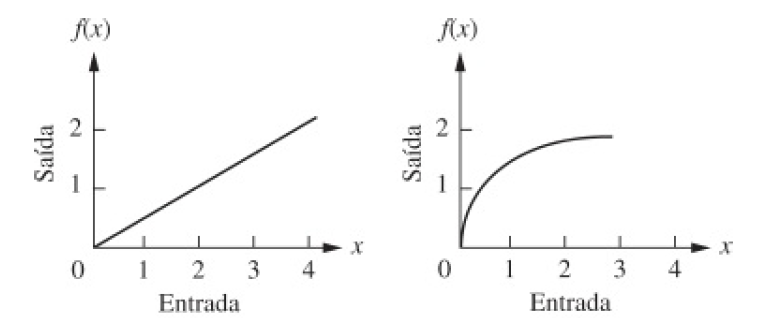
\includegraphics[width=0.9\linewidth]{Figuras/Ch13/fig7.PNG}}
}

\frame{
\frametitle{Introdução}
\begin{block}{Sistemas não lineares}
\begin{itemize}
    \item Embora muitas relações de grandezas físicas sejam representadas por equações lineares, na maioria dos casos a relação entre elas \textbf{não é efetivamente linear}.
    \item Os sistemas são realmente \textbf{lineares} somente para \textbf{intervalos limitados de operação}.
    \item \textbf{Exemplo:} amortecedores utilizados em sistemas físicos podem ser lineares para operações de baixa velocidade, mas podem ser tornar não lineares para velocidades elevadas.
\end{itemize}
\end{block}
}

\frame{
\frametitle{Não linearidades}
\begin{block}{Exemplo $\#01$}
\begin{itemize}
    \item Um amplificador eletrônico é linear sobre uma faixa específica de valores, porém apresenta a não linearidade denominada \textbf{saturação} para tensões de entrada elevadas.
\end{itemize}
\end{block}
\centerline{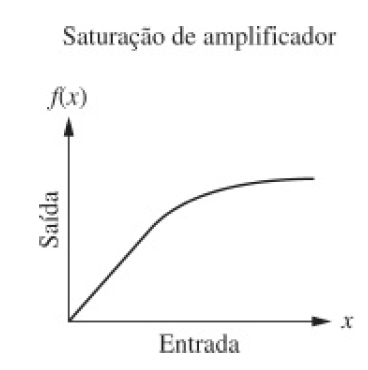
\includegraphics[width=0.4\linewidth]{Figuras/Ch13/fig1.PNG}}
}

\frame{
\frametitle{Não linearidades}
\begin{block}{Exemplo $\#02$}
\begin{itemize}
    \item Um motor que não responde a tensões de entrada muito baixas, devido às forças de atrito, apresenta uma não linearidade denominada \textbf{zona morta}.
\end{itemize}
\end{block}
\centerline{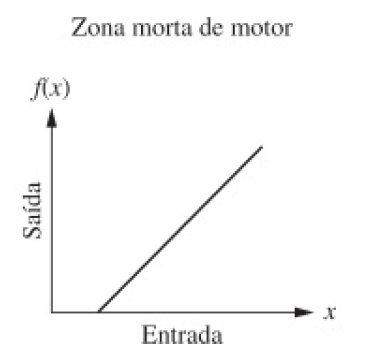
\includegraphics[width=0.4\linewidth]{Figuras/Ch13/fig2.PNG}}
}

\frame{
\frametitle{Não linearidades}
\begin{block}{Exemplo $\#03$}
\begin{itemize}
    \item Engrenagens que não se ajustam firmemente apresentam uma não linearidade denominada \textbf{folga}: a entrada se move sobre uma pequena faixa sem que a saída responda.
\end{itemize}
\end{block}
\centerline{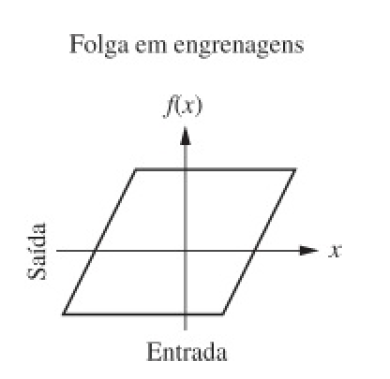
\includegraphics[width=0.4\linewidth]{Figuras/Ch13/fig3.PNG}}
}

\frame{
\frametitle{Linearização}
\begin{block}{Introdução}
\begin{itemize}
    \item A \textbf{aproximação linear} de um sistema não linear simplifica a análise e o projeto de um sistema, desde que os resultados forneçam uma \textbf{boa aproximação} da realidade.
    \item Uma relação linear pode ser estabelecida em um \textbf{ponto} da curva não linear se a faixa de variação dos valores de entrada em torno desse ponto for pequena e se a origem for transladada para esse ponto.
\end{itemize}
\end{block}
}

\frame{
\frametitle{Linearização}
\begin{block}{Ponto de equilíbrio}
\begin{itemize}
    \item Uma operação normal do sistema pode estar em torno de um \textbf{ponto de equilíbrio}.
    \item Se o sistema operar em torno de um ponto de equilíbrio e os sinais envolvidos forem pequenos, então é possível \textbf{aproximar} o sistema não linear por um sistema linear.
    \item \textbf{Exemplo:} quando um pêndulo está em repouso ele está em \textit{equilíbrio}. O deslocamento angular é descrito por uma equação diferencial não linear, porém ele pode ser expresso por uma \textbf{equação diferencial linear} para pequenas variações em torno deste ponto de equilíbrio.
\end{itemize}
\end{block}
}

\frame{
\frametitle{Linearização}
\begin{block}{Passos para a linearização}
\begin{enumerate}
    \item \textbf{Identificar} o componente não linear.
    \item Escrever a \textbf{equação diferencial não linear}.
    \item Escolher o \textbf{ponto de equilíbrio}.
    \item \textbf{Linearizar} a equação diferencial não linear.
    \item Aplicar a \textbf{transformada de Laplace} à equação diferencial linearizada, admitindo condições iniciais nulas.
    \item Separar as variáveis de entrada e saída para formar a \textbf{função de transferência}.
\end{enumerate}
\end{block}
}

\frame{
\frametitle{Linearização - abordagem gráfica}
\begin{block}{Método}
\begin{itemize}
    \item Considere um sistema não linear operando em um \textbf{ponto} $A$, $[x_0,f(x_0)]$
\end{itemize}
\end{block}
\centerline{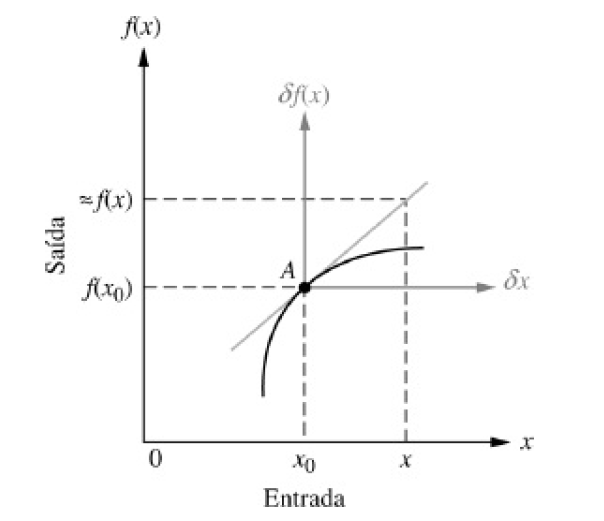
\includegraphics[width=0.5\linewidth]{Figuras/Ch13/fig4.PNG}}
}

\frame{
\frametitle{Linearização - abordagem gráfica}
\begin{block}{Método}
\begin{itemize}
    \item Se a \textbf{inclinação da curva} no ponto $A$ é $m_a$, então pequenas variações da entrada em torno do ponto $A$, $\delta x$, produzem pequenas variações na saída, $\delta f(x)$, relacionadas pela inclinação no ponto $A$.
\end{itemize}
\end{block}
\centerline{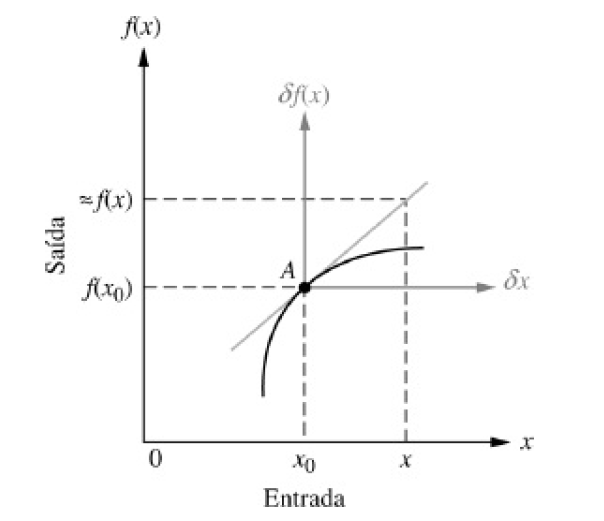
\includegraphics[width=0.5\linewidth]{Figuras/Ch13/fig4.PNG}}
}

\frame{
\frametitle{Linearização - abordagem gráfica}
\begin{block}{Método}
$$[f(x) - f(x_0)] \approx m_a(x - x_0) \implies \delta f(x) \approx m_a \delta x$$
Com isso,
$$f(x) \approx f(x_0) + m_a(x - x_0) \approx f(x_0) + m_a \delta x$$
\begin{itemize}
    \item Um novo conjunto de eixos, $\delta x$ e $\delta f(x)$, é criado com a origem no ponto $A$, e $f(x)$ é aproximadamente igual a $f(x_0)$, a ordenada da \textbf{nova origem}, somada a pequenas excursões, $m_a \delta x$, a partir do ponto $A$.
\end{itemize}
\end{block}
}

\frame{
\frametitle{Exemplo $\#01$ - linearização por abordagem gráfica}
\begin{block}{Problema}
Linearize $f(x) = 5 \ cos(x)$ em torno de $x = \pi/2$.
\end{block}
\centerline{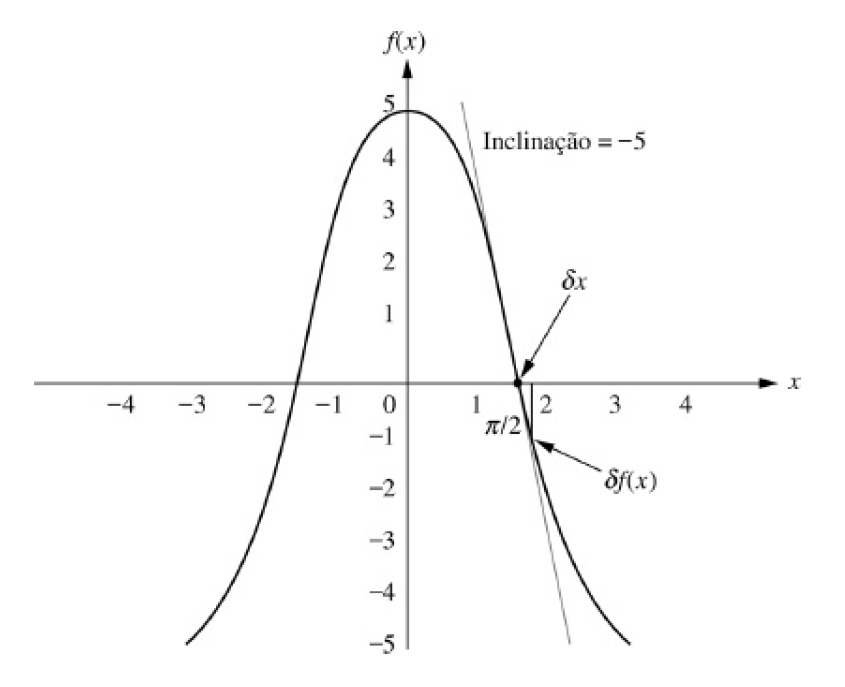
\includegraphics[width=0.65\linewidth]{Figuras/Ch13/fig5.PNG}}
}

\frame{
\frametitle{Exemplo $\#01$ - linearização por abordagem gráfica}
\begin{block}{Solução}
\begin{itemize}
    \item Para descobrir a inclinação da curva no ponto $A$, deve-se fazer a \textbf{derivada} da função no ponto $x_0$.
\end{itemize}
$$m_a = \dfrac{df}{dx}\Big|_{x_0=\pi/2} = -5 \ sen(x)\Big|_{x_0=\pi/2} = -5$$
\begin{itemize}
    \item Além disso, $f(x_0) = f(\pi/2) = 5 \ cos(\pi/2) = 0$
\end{itemize}
Deste modo,
$$f(x) \approx f(x_0) + m_a \delta x \approx -5 \delta x$$
para pequenas variações de $x$ em torno de $\pi/2$.
\end{block}
}

\frame{
\frametitle{Linearização - série de Taylor}
\begin{block}{Método}
\begin{itemize}
    \item \textbf{Formalização} da abordagem gráfica.
    \item A série de Taylor expressa o valor de uma função em termos do valor dessa função em um \textbf{ponto particular}, da variação em \textbf{torno desse ponto} e das \textbf{derivadas} calculadas nesse ponto.
\end{itemize}
$$f(x) = f(x_0) + \dfrac{df}{dx}\Big|_{x = x_0} \dfrac{(x - x_0)}{1!} + \dfrac{d^2f}{dx^2}\Big|_{x = x_0} \dfrac{(x - x_0)^2}{2!} + \cdots$$
\begin{itemize}
    \item Para pequenas variações de $x$ em torno de $x_0$ podemos \textbf{desprezar os termos de ordem superior}.
    \item A aproximação resultante fornece uma relação na forma de uma \textbf{reta} entre a variação em $f(x)$ e as variações em torno de $x_0$.
\end{itemize}
\end{block}
}

\frame{
\frametitle{Linearização - série de Taylor}
\begin{block}{Método}
Deste modo,
$$f(x) - f(x_0) \approx \dfrac{df}{dx}\Big|_{x = x_0} (x - x_0)$$
Com isso,
$$\boxed{\delta f(x) \approx m\big|_{x = x_0} \delta x}$$
\end{block}
}

\frame{
\frametitle{Exemplo $\#01$ - linearização pela série de Taylor}
\begin{block}{}
Linearize a EDO abaixo para pequenas variações em torno de $x = \pi/4$.
$$\dfrac{d^2x}{dt^2} + 2 \dfrac{dx}{dt} + cos \ x = 0$$ \\
\vspace{0.2cm}
\textbf{Resolução:} \\
\vspace{0.2cm}
Uma vez que desejamos linearizar a equação em torno de $x = \pi/4$, fazemos $x = \delta x + \pi/4$, em que $\delta x$ é a pequena variação em torno de $\pi/4$, e substituímos $x$. Logo,
$$\dfrac{d^2(\delta x + \pi/4)}{dt^2} + 2 \dfrac{d(\delta x + \pi/4)}{dt} + cos \ (\delta x + \pi/4) = 0$$
$$\dfrac{d^2\delta x}{dt^2} + 2 \dfrac{d\delta x}{dt} + cos \ (\delta x + \pi/4) = 0$$
\end{block}
}

\frame{
\frametitle{Exemplo $\#01$ - linearização pela série de Taylor}
\begin{block}{}
O termo $cos \ (\delta x + \pi/4)$ pode ser linearizado pela série de Taylor.
$$f(x) - f(x_0) \approx \dfrac{df}{dx}\Big|_{x = x_0} (x - x_0)$$
$$cos \ (\delta x + \pi/4) - cos(\pi/4) \approx \dfrac{d \ cos \ x}{dx}\Big|_{x = \pi/4} \delta x$$
Deste modo,
$$cos \ (\delta x + \pi/4) \approx cos(\pi/4) - sen(\pi/4) \delta x \approx \dfrac{\sqrt{2}}{2} - \dfrac{\sqrt{2}}{2} \delta x$$
A EDO linearizada fica, portanto:
$$\dfrac{d^2\delta x}{dt^2} + 2 \dfrac{d\delta x}{dt} - \dfrac{\sqrt{2}}{2} \delta x = - \dfrac{\sqrt{2}}{2}$$
Esta equação pode agora ser resolvida para $\delta x$, de onde podemos obter $x = \delta x + \pi/4$.
\end{block}
}

\frame{
\frametitle{Exemplo $\#02$ - linearização pela série de Taylor}
\begin{block}{Problema}
Determine a função de transferência $V_L(s)/V(s)$ para o circuito elétrico abaixo, que contém um resistor não linear cuja relação corrente-tensão é definida por $i_r = 2e^{0,1v_r}$. Além disso, $v(t)$ é uma fonte de pequenos sinais.
\end{block}
\vspace{0.3cm}
\centerline{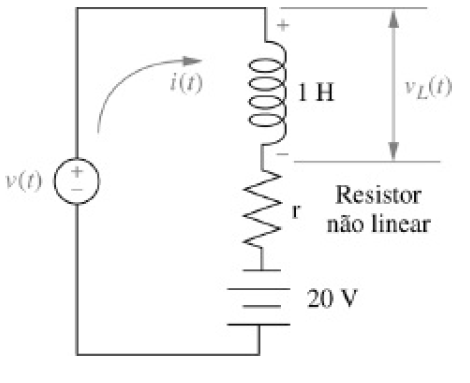
\includegraphics[width=0.5\linewidth]{Figuras/Ch13/fig6.PNG}}
}

\frame{
\frametitle{Exemplo $\#02$ - linearização pela série de Taylor}
\begin{block}{Resolução}
\begin{itemize}
    \item O primeiro passo é obter a relação tensão-corrente sobre o resistor não linear.
\end{itemize}
$$i_r = 2e^{0,1v_r} \implies v_r = 10 \ \text{ln} \dfrac{1}{2}i_r$$
\begin{itemize}
    \item Aplicando a LKT na malha única, e lembrando que $i_r = i$, vem:
\end{itemize}
$$L \dfrac{di}{dt} + 10 \ \text{ln} \dfrac{1}{2}i - 20 = v(t)$$
\begin{itemize}
    \item Para calcular o ponto de equilíbrio, devemos fazer a fonte de pequenos sinais, $v(t)$, igual a zero -- e após isto, calcular a corrente em regime permanente.
    \begin{itemize}
        \item No regime permanente a tensão no indutor será nula.
        \item A tensão no resistor, $v_r$, é 20 V.
        \item $i_r = 2e^{0,1v_r} = i = i_0 = \SI{14,78}{\ampere}$.
    \end{itemize}
\end{itemize}
\end{block}
}

\frame{
\frametitle{Exemplo $\#02$ - linearização pela série de Taylor}
\begin{block}{Resolução}
Com isso, $i = \delta i + i_0$.
Deste modo,
$$L \dfrac{d(\delta i + i_0)}{dt} + 10 \ \text{ln} \dfrac{1}{2}(\delta i + i_0) - 20 = v(t)$$
O termo $\text{ln} \dfrac{1}{2}(\delta i + i_0)$ pode ser linearizado pela série de Taylor.
$$f(i) - f(i_0) \approx \dfrac{df}{di}\Big|_{i = i_0} (i - i_0)$$
$$\text{ln} \dfrac{1}{2}(\delta i + i_0) - \text{ln} \dfrac{1}{2}(i_0) \approx \dfrac{d \ (\text{ln} \tfrac{1}{2} i)}{di}\Big|_{i = 14,78} \delta i$$
Deste modo,
$$\text{ln} \dfrac{1}{2}(\delta i + 14,78) \approx \text{ln} \dfrac{1}{2}(14,78) + \dfrac{1}{14,78} \delta i \approx 2 + 0,0677 \delta i$$
\end{block}
}

\frame{
\frametitle{Exemplo $\#02$ - linearização pela série de Taylor}
\begin{block}{Resolução}
A EDO linearizada fica, portanto:
$$\dfrac{d\delta i}{dt} + 10 (2 + 0,0677 \delta i) - 20 = v(t)$$
Simplificando, obtemos:
$$\dfrac{d\delta i}{dt} + 0,677 \delta i = v(t)$$
Aplicando a transformada de Laplace com condições inicias nulas:
$$\delta i(s) = \dfrac{V(s)}{s + 0,677}$$
\end{block}
}

\frame{
\frametitle{Exemplo $\#02$ - linearização pela série de Taylor}
\begin{block}{Resolução}
A tensão sobre o indutor em torno do ponto de equilíbrio é
$$V_L(t) = L \dfrac{d}{dt}(i_0 + \delta i) = L \dfrac{d \delta i}{dt}$$
Aplicando a transformada de Laplace com condições inicias nulas:
$$V_L(s) = Ls \delta i(s) = s \delta i(s)$$
Com isso,
$$V_L(s) = s \delta i(s) = s \cdot \dfrac{V(s)}{s + 0,677}$$
Rearrumando, chegamos ao resultado final:
$$\dfrac{V_L(s)}{V(s)} = \dfrac{s}{s+0,677}$$
para pequenas variações em torno de $i = \SI{14,78}{\ampere}$.
\end{block}
}

\frame{
\frametitle{Exemplo $\#03$ - linearização pela série de Taylor}
\begin{block}{}
Obtenha o modelo linearizado de um sistema massa-mola-amortecedor cuja mola possui característica não linear $f_K(x) = -(x-20)^2+400$, no qual $x=0$ corresponde a mola sem compressão ou distensão. Considere que $f_K(x)$ é válido no intervalo $[-10,10]$. \\
\vspace{0.4cm}
\textbf{Resolução:} \\
\vspace{0.4cm}
O modelo não linear é dado por:
$$M \ddot{x} + B \dot{x} + f_K(x) = f_a(t)$$
Logo,
$$M \ddot{x} + B \dot{x} -(x-20)^2+400 = f_a(t)$$
Descobrimos o ponto de operação igualando $f_K(x) = 0$. Deste modo,
$$-(x-20)^2+400 = 0 \implies x = 0 \ \text{(pertencente ao intervalo)}$$
\end{block}
}

\frame{
\frametitle{Exemplo $\#03$ - linearização pela série de Taylor}
\begin{block}{}
Uma vez que desejamos linearizar a equação em torno de $x = 0$, fazemos $x = \delta x + 0 = \delta x$, em que $\delta x$ é a pequena variação em torno de $0$, e substituímos $x$. Logo,
$$M\dfrac{d^2\delta x}{dt^2} + B \dfrac{d\delta x}{dt} -(\delta x-20)^2+400 = f_a(t)$$
\end{block}
}

\frame{
\frametitle{Exemplo $\#03$ - linearização pela série de Taylor}
\begin{block}{}
O termo $-(\delta x-20)^2+400$ pode ser linearizado pela série de Taylor.
$$f(x) - f(x_0) \approx \dfrac{df}{dx}\Big|_{x = x_0} (x - x_0)$$
$$-(\delta x-20)^2+400 - 0 \approx \dfrac{d}{dx}(-(x-20)^2+400)\Big|_{x = 0} \delta x$$
Deste modo,
$$-(\delta x-20)^2+400 \approx -2(0-20) \delta x \approx 40 \delta x$$
A EDO linearizada fica, portanto:
$$M\dfrac{d^2\delta x}{dt^2} + B \dfrac{d\delta x}{dt} + 40 \delta x = f_a(t)$$
Esta equação pode agora ser resolvida para $\delta x$, de onde podemos obter $x = \delta x$.
\end{block}
}

\frame{
\frametitle{Exercícios}
\begin{block}{}
01. Determine a função de transferência linearizada, $G(s) = V(s)/I(s)$, para o circuito elétrico abaixo. O circuito contém um resistor não linear cuja relação corrente-tensão é definida por $i_r = e^{v_r}$. A fonte de corrente, $i(t)$, é um gerador de pequenos sinais.
\end{block}
\centerline{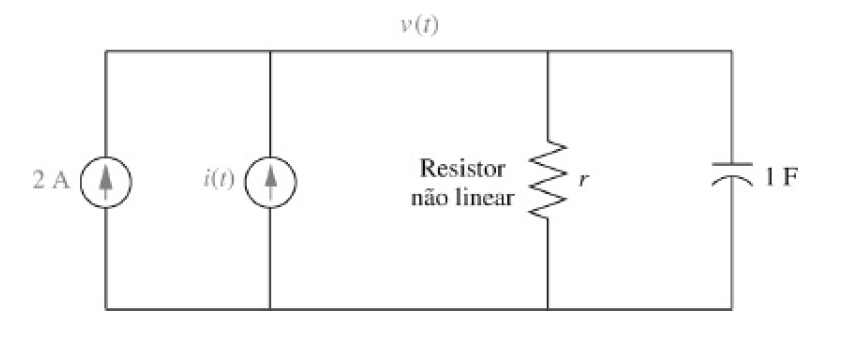
\includegraphics[width=0.8\linewidth]{Figuras/Ch13/fig8.PNG}}
}

\frame{
\frametitle{Referências e exercícios complementares}
\begin{itemize}
\item NISE, Norman S. Engenharia de Sistemas de Controle, 7 ed. LTC, 2017.
\end{itemize}
\centering{\alert{Página 77 - \textbf{Capítulo 2}}}
}